% !Mode:: "TeX:UTF-8"

\chapter{系统测试与分析}

为了证实GPSA系统的实际性能,本章对该系统进行了测试和分析。首先从硬件、软件以及用作测试的数据集三方面介绍了测试环境;接着介绍在GPSA中PageRank、连通分量和广度搜索三个应用的实现,测试它们在不同数据集上的运行性能,并将结果与GraphChi和X-Stream进行对比分析;最后,从对单机多核的利用率角度对系统进行测试和分析。


\section{实验环境}

\subsection{硬件环境}
本文的系统与测试都是运行在相同的计算机上。该计算机CPU为32核,主频1.8GHZ的Intel i7 cores, 16GB内存,1TB硬盘,转速7200rpm。
\subsection{软件环境}
本文的操作系统为Ubuntu 12.04LTS,JDK7,Kilim。另外,本文用来对比的单机图处理系统分别为GraphChi(0.2.6 C++)与X-Stream。

\subsection{测试数据集}
为了能够全面的了解GPSA的运行性能,所以我们选择四个大小不同的数据集:Google数据集、soc-pokec数据集、soc-liveJournal数据集以及twitter-2010数据集。四个数据集的大小情况如下表所示:
\renewcommand\arraystretch{1.5}%控制行距
\begin{table}[!h]
\caption{测试数据集大小}\label{tab:bench}
\vspace{0.5em}
\centering
\begin{tabular}{l*{1}{C{2cm}}*{1}{L{6.2cm}}}
\toprule
Name         & Nodes & Edges\\
\midrule
google      & 875,713  & 5,105,039\\
soc-pokec      & 1,632,803 & 30,622,564\\
soc-liveJournal      & 4,847,571 & 68,993,773\\
twitter-2010      & 41,652,230 & 1,468,365,182\\

\bottomrule
\end{tabular}
\vspace{\baselineskip}
\end{table}
\renewcommand\arraystretch{1}

\section{应用}
在GPSA的框架上实现应用会非常简单,一般情况下只需要实现\textit{Handler}接口,在该接口必须要实现的函数有两个:\textnormal{init(sequence)}和\textnormal{compute(val,msgVal,args)}。其中,\textnormal{init}函数主要用于初始化顶点的状态信息,而compute方法则用于在计算Actor处理消息时进行调用。除此之外,还有一些可选函数,例如消息生成函数、更新判定等,如果不实现这些可选函数,则会以默认方式进行计算。例如,若不实现消息生成函数,则默认将顶点的最新状态打包进消息中进行发送。

\subsection{PageRank}
PageRank是著名的网页排名算法。在GPSA中实现该算法,需要实现\textit{Handler}接口,将顶点的初始值初始化为1.0,然后当计算Actor接收到消息进行计算时,需要对这些消息进行累加,如算法\ref{al:pr}所示。
\begin{algorithm}
{
{
\renewcommand\baselinestretch{1.5}\selectfont %控制行距

\caption{PageRank}
\label{al:pr}
\begin{algorithmic}[1]
\REQUIRE ~\\
	$val,msgVal,args$
\ENSURE ~\\
	$newVal$
\IF{$args[0]$}
	 \RETURN $ 0.15f$
\ENDIF
\RETURN $0.85*msgVal + vertexVal$

\end{algorithmic}
}
\par}
\end{algorithm}

\subsection{BFS}
BFS是对图进行广度遍历的算法。在GPSA中实现该算法则需要指定起始遍历的顶点,起始顶点的值初始化为0,其他顶点初始化为无穷大,通过发送消息并对消息进行计算可以得到某一个顶点在广度遍历中在整个图中的遍历层次。对于一个顶点而言,假如\textit{V}所处的层次为n,那么它的出边的顶点的层次在没有其他干扰情况下(例如,这些顶点同时也是层次为n-1的顶点的出边目的顶点)是n+1。否则,可以通过比较他的目的顶点的层次与它的消息中的新层次,最小的那个即为其在广度遍历算法中的层次。由于无法保证消息的发送和接收顺序,所以在计算函数中通过比较消息的值的层次的大小,并将值最小的消息加1之后作为返回值,具体实现如算法\ref{al:bfs}。
\begin{algorithm}
{
{
\renewcommand\baselinestretch{1.5}\selectfont %控制行距

\caption{Breadth First Search}
\label{al:bfs}
\begin{algorithmic}[1]
\REQUIRE ~\\
	$val,msgVal,args$
\ENSURE ~\\
	$newVal$
\IF{$msgVal < val$}
	 \RETURN $ msgVal + 1$
\ENDIF
\RETURN $val$

\end{algorithmic}
}
\par}
\end{algorithm}
\subsection{CC}
联通分量的实现过程与广度搜索类似,但是在初始化的时候,将所有顶点的值初始化为其自身\textit{id},然后在计算函数中通过比较两者的\textit{id}的大小,选择返回较小值。这样,计算完成
之后,处在同一个连通分量中的顶点拥有相同的\textit{id},具体实现如算法\ref{al:cc}所示。
\begin{algorithm}
{
{
\renewcommand\baselinestretch{1.5}\selectfont %控制行距

\caption{CC}
\label{al:cc}
\begin{algorithmic}[1]
\REQUIRE ~\\
	$val,msgVal,args$
\ENSURE ~\\
	$newVal$
\IF{$msgVal < val$}
	 \RETURN $ msgVal$
\ENDIF
\RETURN $val$

\end{algorithmic}
}
\par}
\end{algorithm}

\section{性能测试}
本文不仅对GPSA系统在不同应用、不同数据集上的表现进行了测试,同时还将之横向与其他单机上的图处理系统进行对比。为保证测试的公正与直观,GPSA、GraphChi和X-Stream均以默认设置运行,通过计算其运行相同步骤所消耗的时间作为性能对比的主要指标。所有的测试都是在同一台计算机上进行,并且分别运行三次其最终的运行时间的平均值。由于GPSA和GraphChi在运行时需要指定运行的迭代次数,而X-Stream则不需要指定该迭代次数。考虑到图计算过程在最开始的若干超级步中的处理速度可以较为直观的反映出计算的效率,因此本文测试了开始前5个超级步的平均消耗时间作为对比的标准。另外,GraphChi和X-Stream的三个测试应用均采用其官方提供的实现。

\subsection{google数据集测试}
图\ref{res:google}展示了三个系统的PageRank、Connect Component和BFS三个不同的应用在Google网图上的运行结果。通过对比可以发现,在PageRank和BFS应用中,GraphChi的性能最好,X-stream次之。在CC应用中,X-Stream的性能最好,GraphChi次之。在PageRank中,GPSA比GraphChi和X-Stream慢大约4倍;在BFS中,GPSA比GraphChi和X-Stream慢大约0.2倍;虽然在CC中,GPSA与GraphChi几乎持平,但是依然比X-Stream慢。

首先,google的数据集相对较小,整个图的文件大小在100MB范围内,可以完全载入内存。GraphChi和X-Stream省去了较多磁盘IO操作,在内存中可以完成所有数据操作。而GPSA由于将图的数据部分保存在磁盘中,所以会有部分的磁盘IO顺序读取。其次,框架的实现有区别。GraphChi和X-Stream使用C/C++实现,而GPSA使用JAVA和Kilim实现,会无可避免的出现垃圾回收等问题,所以在语言效率上,GPSA略逊一筹。

\begin{figure}[htbp]
\centering
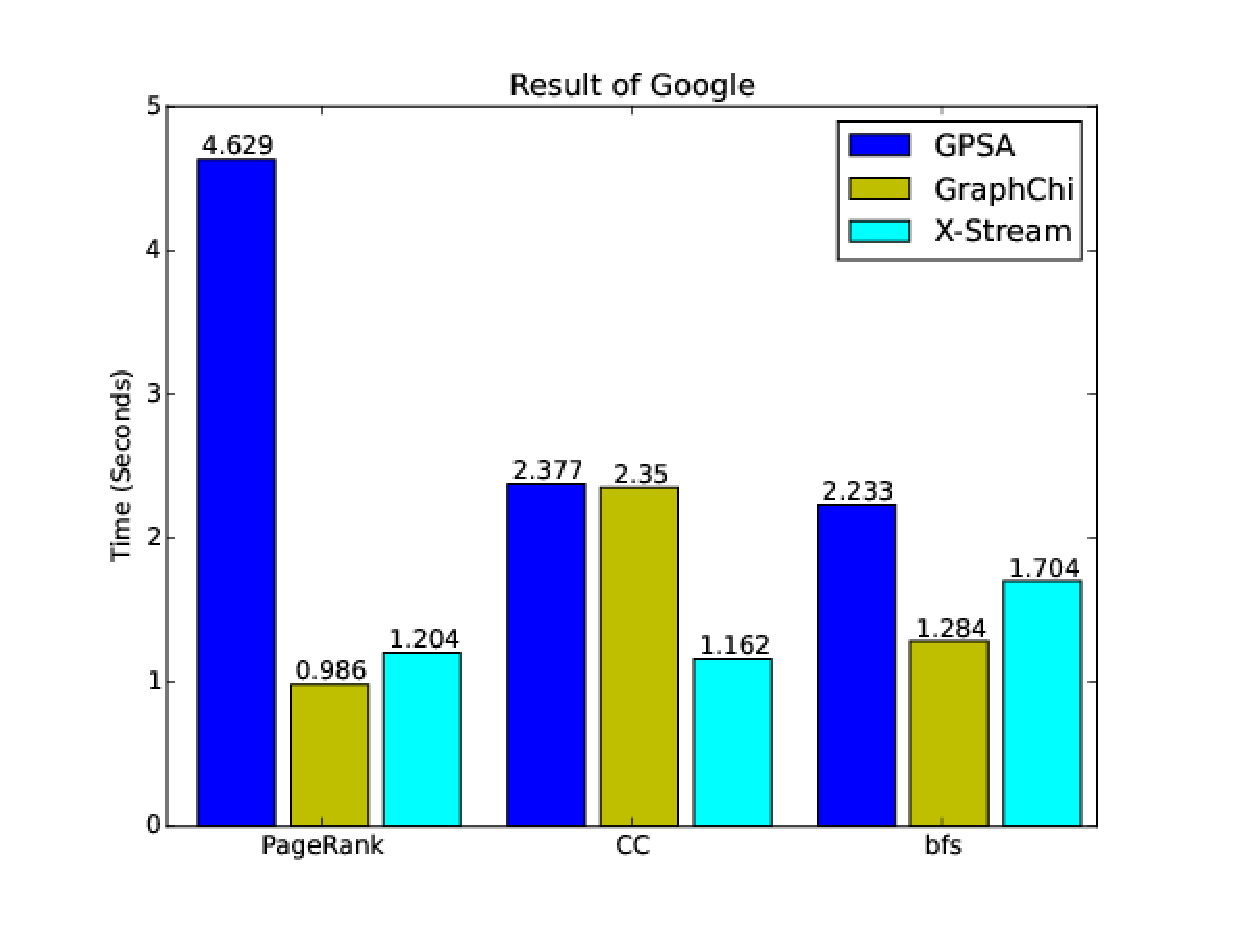
\includegraphics[width=0.6\textwidth,scale=0.8]{myfigures/googletime2.eps}
\caption{Google测试结果}
\label{res:google}
\end{figure}

% \begin{figure}[htbp]
% \centering
% 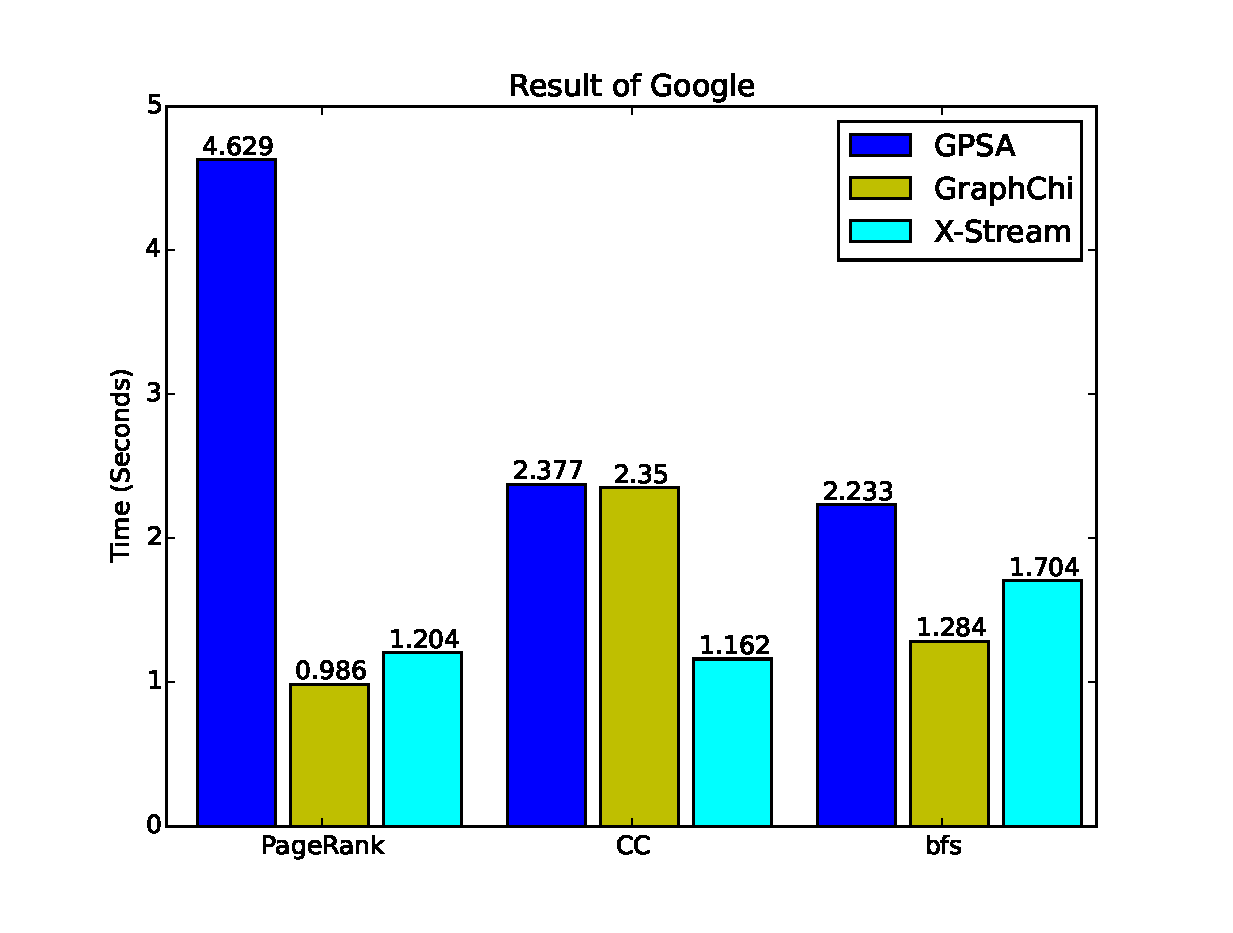
\includegraphics[width=0.4\textwidth]{myfigures/googletime.eps}
% \caption{数据更新}\label{fig:vu}
% \vspace{\baselineskip}
% \end{figure}


\subsection{soc-数据集测试}
图\ref{res:pokec}展示了GPSA、GraphChi和X-Stream在soc-Pokec数据集上分别运行PageRank、Connect Component和BFS三个应用的运行结果。通过对比实验结果可以发现,GPSA的性能最好,GraphChi次之。在PageRank中,GPSA比GraphChi快大约0.3倍,比X-Stream快8倍;在CC中,GPSA比GraphChi快大约4倍,比X-Stream快约6倍;在BFS中,GPSA与GraphChi几乎持平,而X-Stream较差。

\begin{figure}[htbp]
\centering
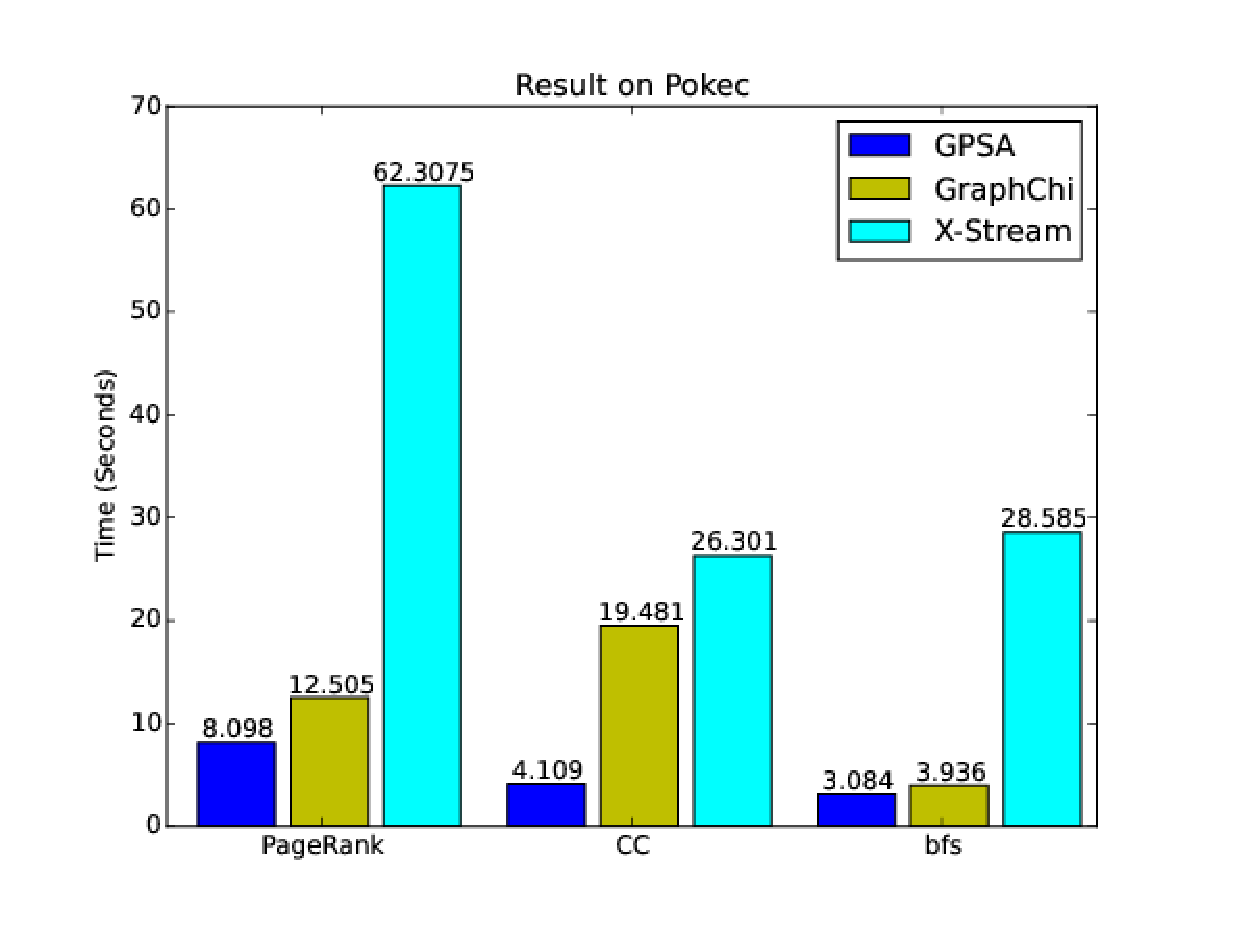
\includegraphics[width=0.6\textwidth,scale=0.8]{myfigures/pokectime2.eps}
\caption{soc-Pokec测试结果}
\label{res:pokec}
\end{figure}


图\ref{res:journal}展示了GPSA、GraphChi和X-Stream在soc-liveJournal数据集上分别运行PageRank、Connect Component和BFS三个应用的运行结果。通过对比实验结果可以发现,GPSA的性能最好,GraphChi次之。在PageRank中,GPSA比GraphChi快大约0.3倍,比X-Stream快10倍;在CC中,GPSA比GraphChi快大约4倍,比X-Stream快约6倍;在BFS中,GPSA与GraphChi几乎持平,而X-Stream较差。

\begin{figure}[htbp]
\centering
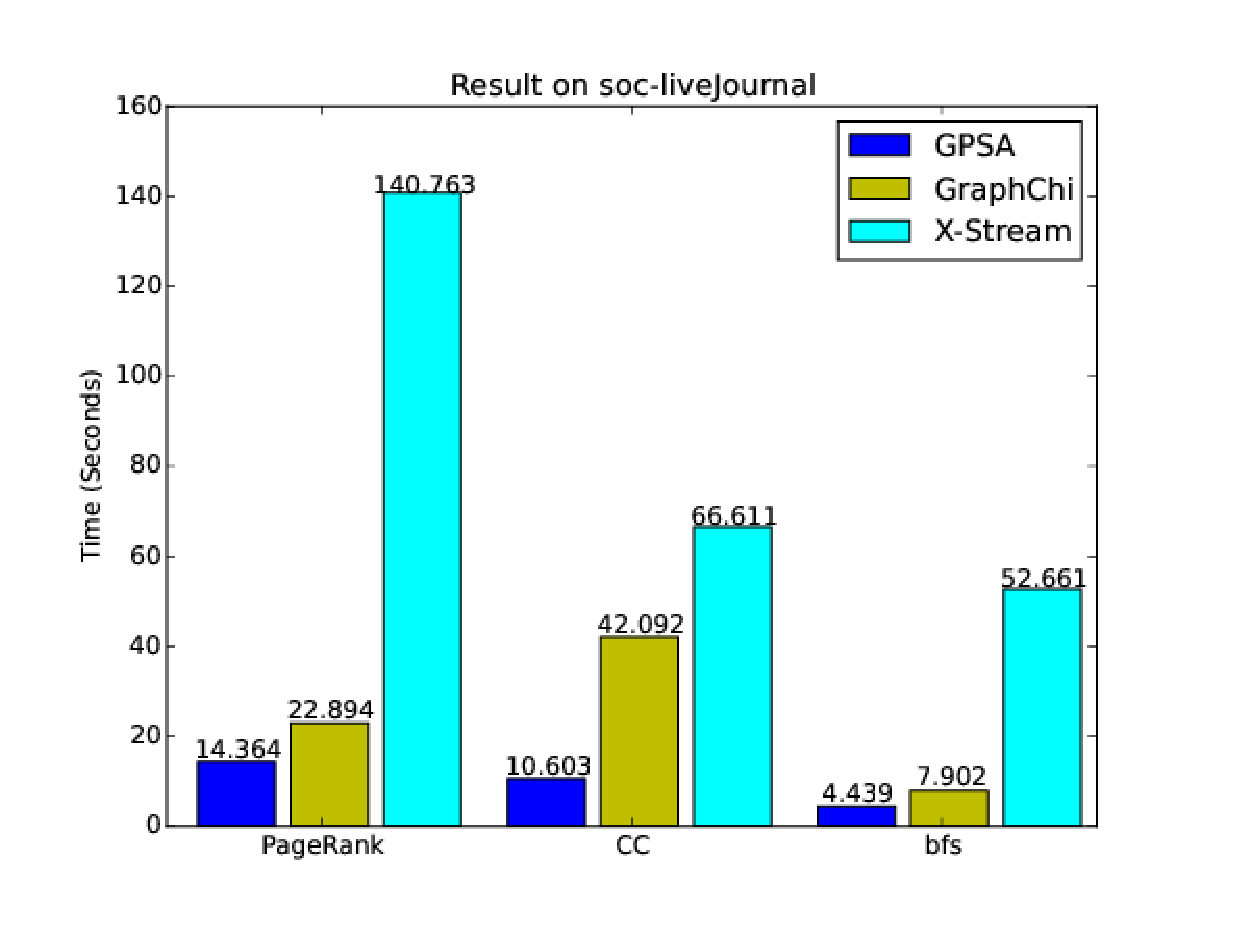
\includegraphics[width=0.6\textwidth,scale=0.8]{myfigures/journaltime2.eps}
\caption{soc-liveJournal测试结果}
\label{res:journal}
\end{figure}

通过\ref{res:pokec}和\ref{res:journal}的实验结果可以发现实验结果具有一定的一致性,GPSA的测试性能与在Google数据上有着巨大的差别。首先,从上文数据集的信息介绍中可以发现soc-Pokec和soc-liveJournal两个数据集都是中等规模大小的图数据,无论是顶点数目还是边的数目都比比Google数据集大的多。因此,GraphChi和X-Stream需要对数据进行分批载入,同时在超级步完成之后,需要写大量的数据到磁盘,引发大量的磁盘IO操作。而GPSA由于无需保存大量的数据到磁盘,所以在超级步更替的时候,无需额外的IO操作,效率较之两者有着明显提高。其次,可以看到GPSA和GraphChi的性能比X-Stream好。这主要是因为X-Stream是以边为中心的模型,所以在每次计算时都需要对所有的边进行迭代,而GraphChi以顶点为中心,在每次计算过程中,对于未发生过更新的顶点会跳过,减少消息量与计算量。虽然在GPSA中将顶点以Actor进行了替换,但是GPSA依然继承了对顶点状态的检查操作,使得与GraphChi有着同样的优势。

\subsection{twitter-2010数据集测试}
图\ref{res:twitter}展示了GPSA、GraphChi和X-Stream在soc-Twitter-2010数据集上分别运行PageRank、Connect Component和BFS三个应用的运行结果。通过对比实验结果可以发现,在PageRank中,GPSA比GraphChi快大约2倍,比X-Stream快8倍;在CC中,GPSA比GraphChi快大约5倍,比X-Stream快约4倍;在BFS中,GPSA比X-Stream快约6倍。(由于GraphChi的官方提供的BFS实现在对数据进行预处理完之后,无法继续运行,所以此处的数据无从得知。)

Twitter2010是一个非常大的数据集。通过对该数据集的测试,
可以充分展示GPSA在性能方面的提升与应对大规模图的计算能力。首先,在设计之初,GPSA将计算过程和分发过程进行分离,以一种重叠的方式并发运行,缩短了BSP模型中在垂直方向上的平均执行时间。其次,GPSA 将图的数据分为易变的顶点信息和不易变的边信息区别对待,部分保存在磁盘上,部分保存在内存中,实现了数据的随机访问,降低IO开销。最后,GPSA中计算Actor和分发Actor的协同工作使得无需保存大量的中间消息,只须关注计算结果,简化了计算过程。

\begin{figure}[htbp]
\centering
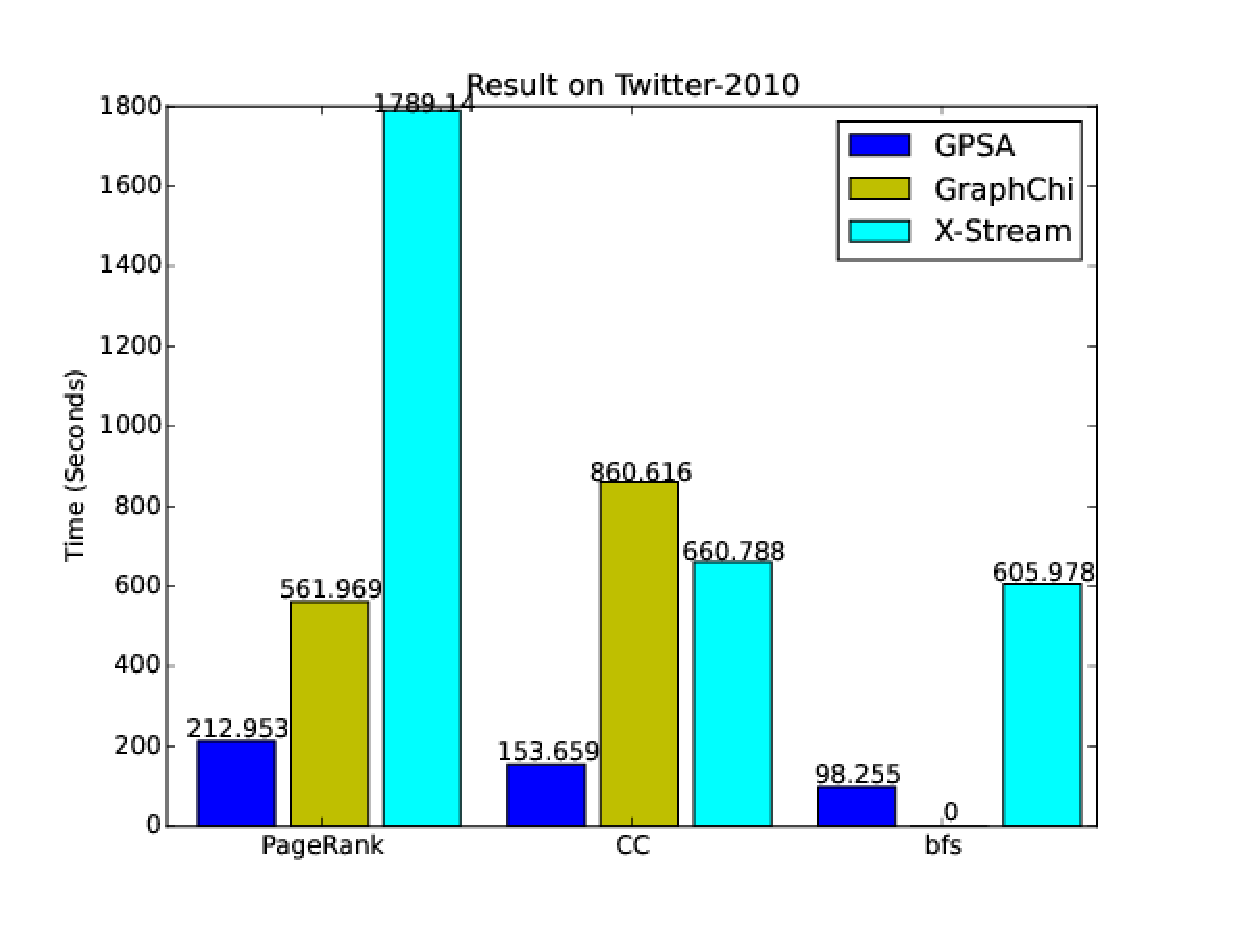
\includegraphics[width=0.6\textwidth,scale=0.8]{myfigures/twittertime2.eps}
\caption{Twitter测试结果}
\label{res:twitter}
\end{figure}


\section{多核利用率测试}
GPSA是为运行在单机多核的系统上而设计的,所以对GPSA进行多核利用率的测试可以直观的了解GPSA。如图\ref{res:usagepr}到\ref{res:usagebfs}所示,比较了GPSA、GraphChi和X-Stream在不同的数据集上,不同的应用上运行时的对多核CPU的利用情况。
\begin{figure}[htbp]
\centering
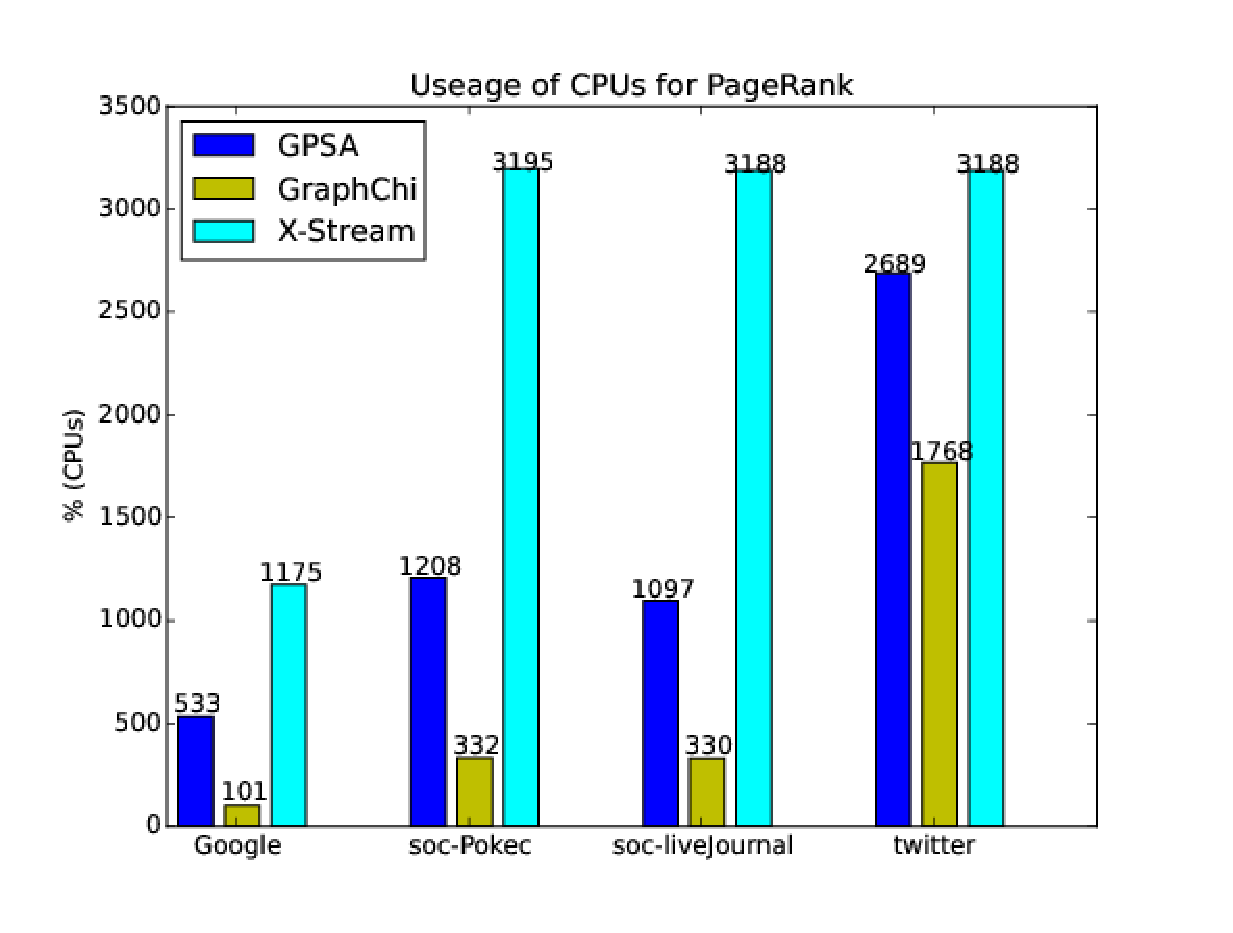
\includegraphics[width=0.6\textwidth,scale=0.8]{myfigures/usagepr2.eps}
\caption{PageRank算法的多核CPU利用率}
\label{res:usagepr}
\end{figure}
\begin{figure}[htbp]
\centering
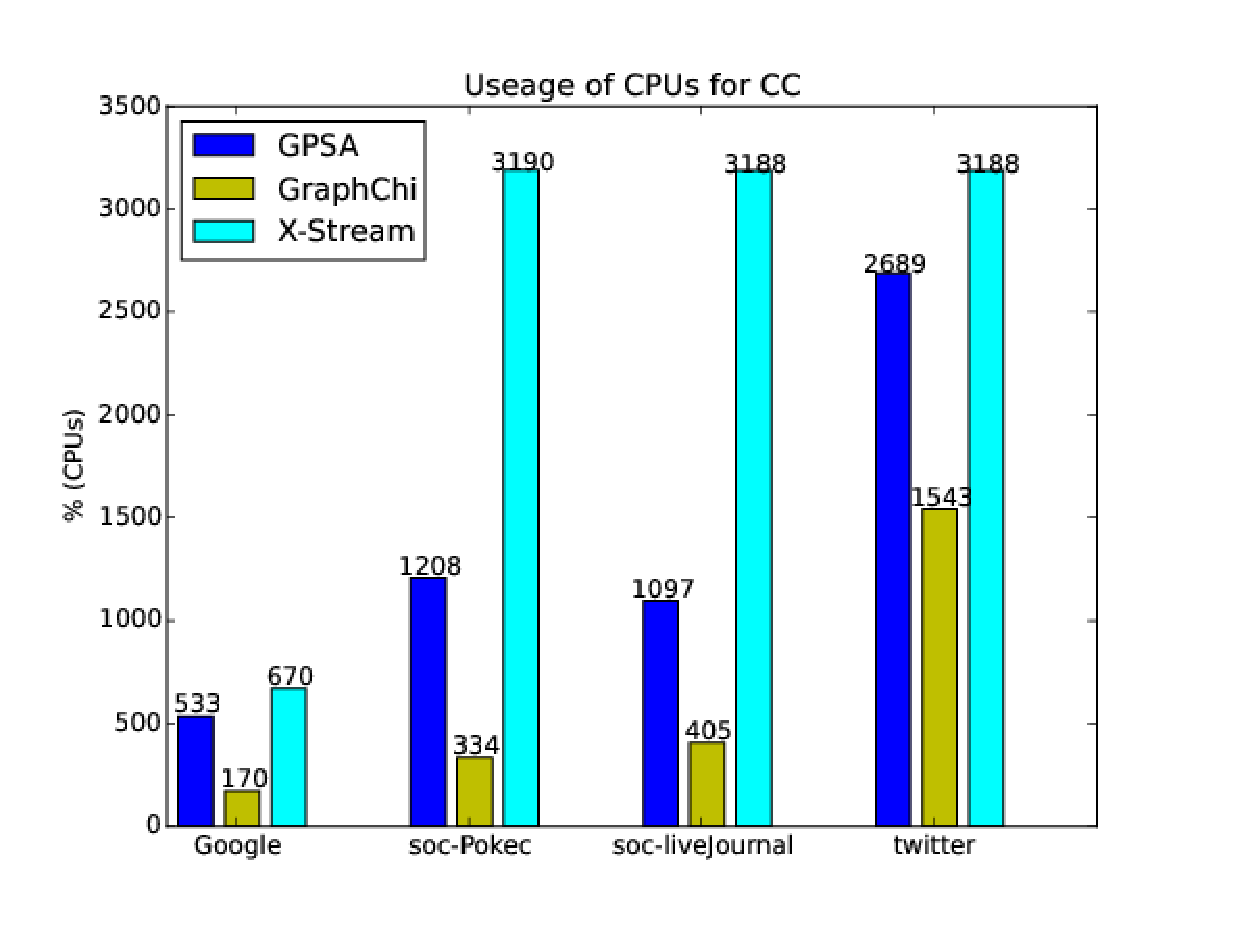
\includegraphics[width=0.6\textwidth,scale=0.8]{myfigures/usagecc2.eps}
\caption{CC算法的多核CPU利用率}
\label{res:usagecc}
\end{figure}
\begin{figure}[htbp]
\centering
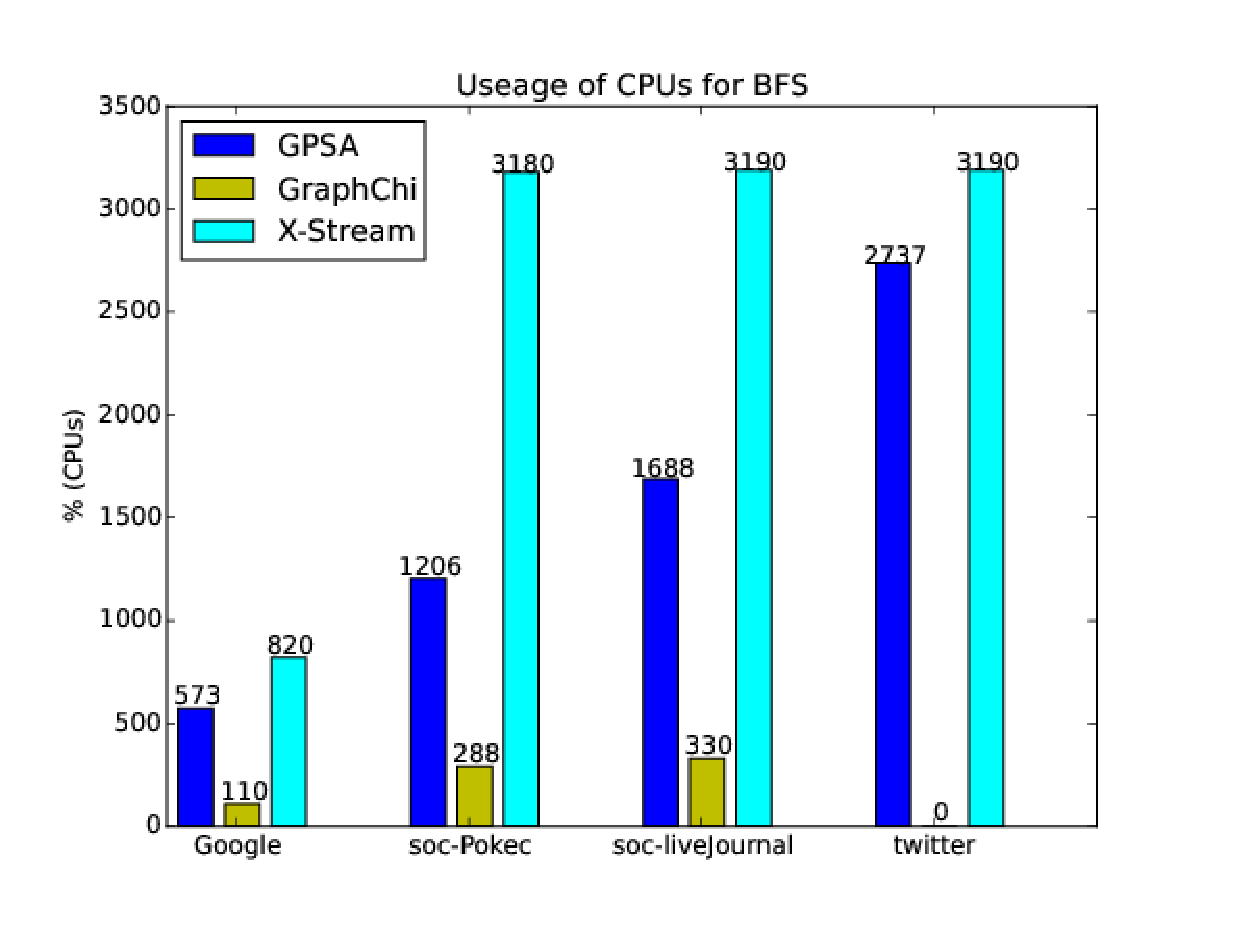
\includegraphics[width=0.6\textwidth,scale=0.8]{myfigures/usagebfs2.eps}
\caption{BFS算法的多核CPU利用率}
\label{res:usagebfs}
\end{figure}


通过测试结果可以直观的发现,X-Stream对多核CPU的利用率最高,GPSA次之,GraphChi则相对较差。GPSA
与GraphChi具有较好的伸缩性与灵活度,对CPU的利用率能够随着应用和数据的不同而灵活的调节,而X-Stream的灵活性和扩展性表现较差,如图\ref{res:usagecc}所示,X-Stream在soc-pokec与twitter两个数据集上都表现出了非常高的CPU利用率,可是相比于twtitter数据集的庞大,soc-pokec数据集的数据量非常小,但是两者的CPU占用情况均高达99\%。反观GraphChi与GPSA,它在处理大小不同的数据集时,对CPU的占用率则呈现出较好的扩展性,例如在图\ref{res:usagepr}中,GPSA在四个应用上对CPU的占用率分别为533\%、1208\%、1097\%、2689\%,当数据量逐步增大时,对CPU的占用率也会相应的增大。

首先,GraphChi的多核CPU的利用率相对较差的主要原因在于GraphChi需要写大量的数据到磁盘,涉及大量频繁的IO操作。虽然X-Stream同样需要写入大量的数据到磁盘,但是X-Stream利用异步IO来充分利用多核CPU的优势。其次,X-Stream具有较差的伸缩性。X-Stream是以边为中心的计算模型,内步实现使用线程并发,虽然利用异步IO提高了效率,但是也导致在无论数据集大小的情况下,CPU总是被时刻占用。
最后,GPSA在三个系统中不仅具有较高的CPU利用率,同时具有较好的伸缩性。这主要得益于GPSA的数据易变与不易变分离以及分发与计算分离,在节省大量IO操作的同时,Actor模型的轻量级并发使得在利用多核并发时相比线程并发而言更具优势。

% \begin{figure}[htbp]
%   \centering
%   \subfigure[PageRank算法的多核CPU利用率]{
%             \label{res:cpu:pr}
%             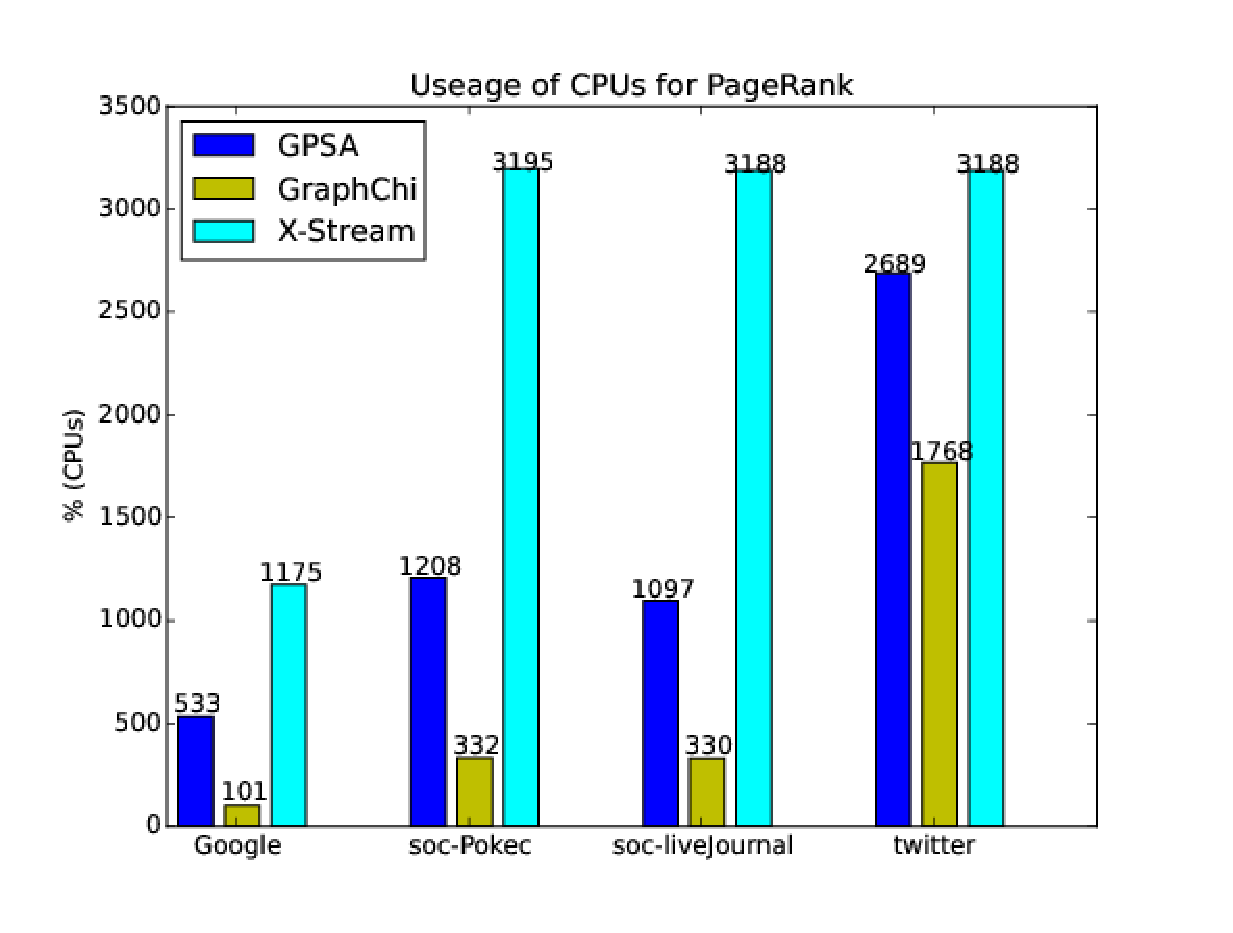
\includegraphics[width=0.4\textwidth]{myfigures/usagepr2.eps}}
%   \subfigure[CC算法的多核CPU利用率]{
%             \label{ res:cpu:cc}
%             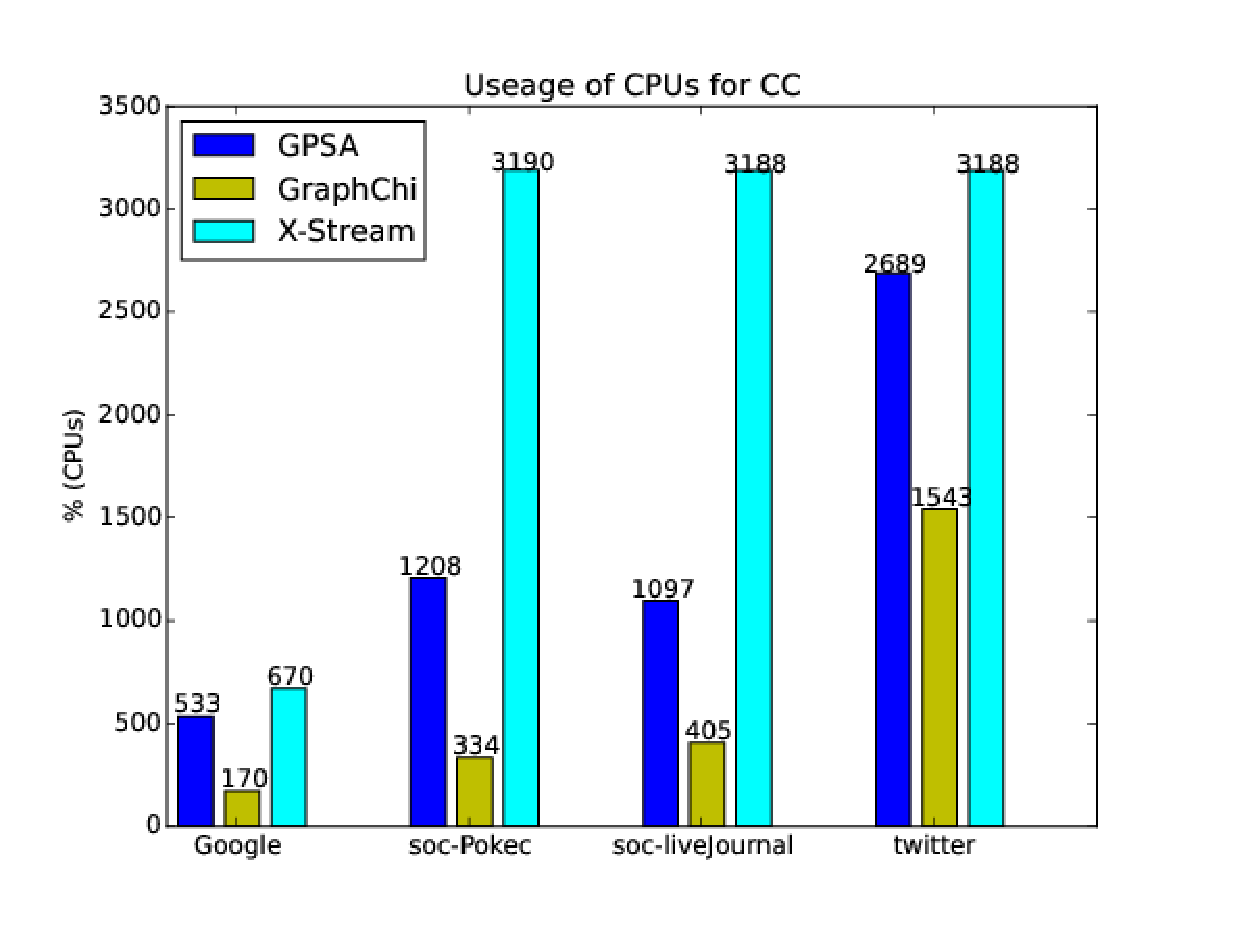
\includegraphics[width=0.4\textwidth]{myfigures/usagecc2.eps}}

%   \subfigure[BFS算法的多核CPU利用率]{
%             \label{res:cpu:bfs}
%             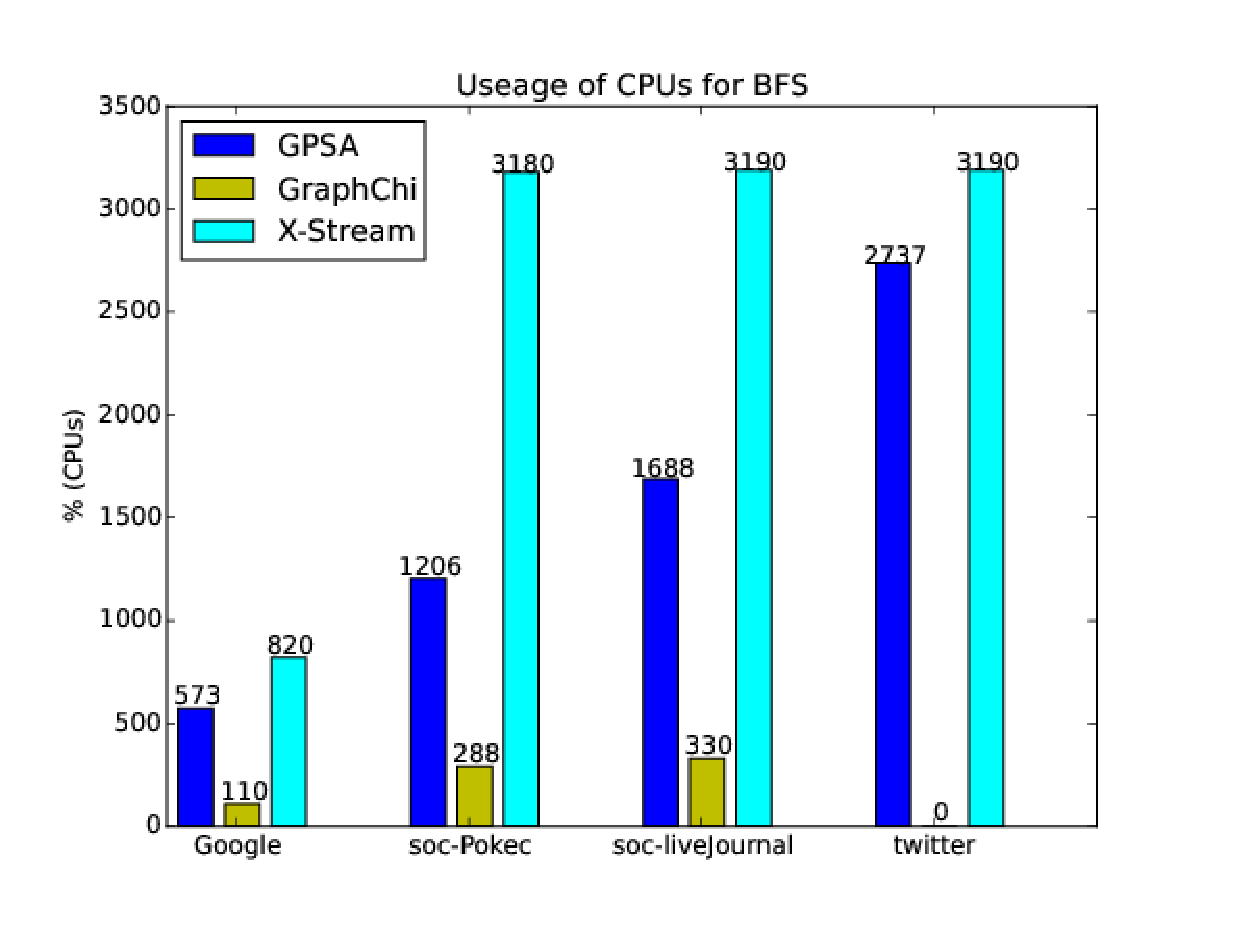
\includegraphics[width=0.4\textwidth]{myfigures/usagebfs2.eps}}

%   \caption{多核CPU利用率}\label{res:cpu}
% \vspace{\baselineskip}
% \end{figure}




\section{小结}






